\section{Mechanical Design}

\subsection{Structure \& Vehicle Layout Overview}


\begin{figure}[H]
\begin{center}
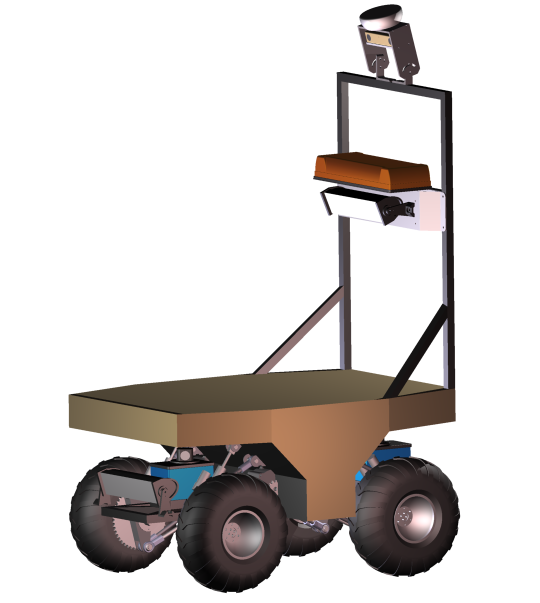
\includegraphics[width=3in]{./Pics/Misti_Vehicle.png}
\caption{Misti, the 2012-2013 Base}

\label{FIG:Misti}
\end{center}
\end{figure}

While the team did moderately well in the 2012 competition, certain areas of improvement were noted and emphasized in this year’s design. Similar to the previous three years, the design revolved around a four-wheeled drive platform, with focus on reducing build complexity and increasing ease of vehicle maintenance (i.e. accessibility to components, proper wire routing, etc.) The team approached the 2013 design with the following goals:

\begin{enumerate}
\item Improve Vehicle Ride Dynamics
\item Increase Ground Clearance
\item Improve Human Interface for Debugging
\item Weatherproofing for Inclement Weather 
\item Enhance Night-Time Operability
\end{enumerate}

By following these goals, the team developed the current vehicle which boasts a vastly superior suspension system and drivetrain, as well as much improved component layout and accessibility.

\subsection{Vehicle Ride Dynamics}
\subsubsection{Drive System}
The vehicle, dubbed Misti, has a completely customized drivetrain designed to deliver high torque for operating on rough terrain.

The two central gearboxes, custom-made and milled from aluminum, are driven by 4.5 peak horsepower Ampflow A28-400 brushed DC motors. Gear reduction comes from a two-stage gear train inside the gearbox, as seen in Figure \ref{FIG:Gearbox}, with the output sprocket driving a chain connected to a sprocket affixed to the wheel, producing a total reduction of 30 to 1. The skid-steer approach was maintained from the previous 3 competitions, but the fore and aft wheels are now mechanically linked together to ensure they maintain the same speed. This ensures that under slippery conditions, the power is always transmitted to the ground through the wheel with the most traction. 

\begin{figure}[H]
\begin{minipage}[b]{0.5\linewidth}
\centering
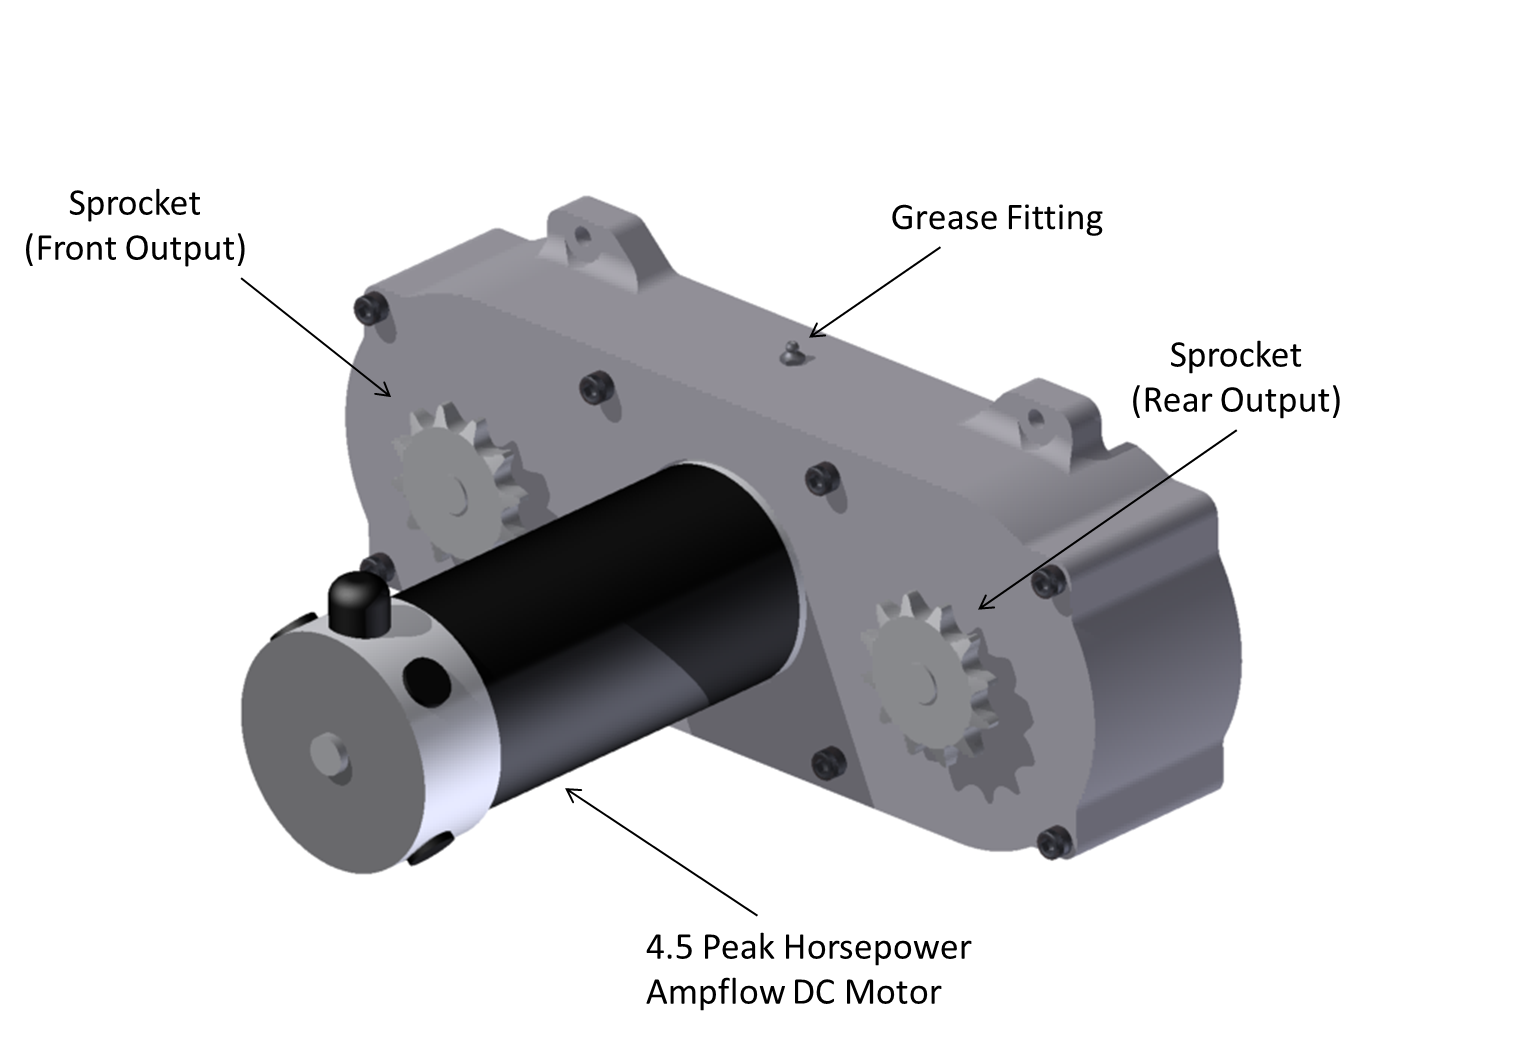
\includegraphics[width=3in]{./Pics/GearboxAssembled.png}
\caption{Custom Gearbox}
\label{FIG:Gearbox}
\end{minipage}
\hspace{0.1in}
\begin{minipage}[b]{0.5\linewidth}
\centering
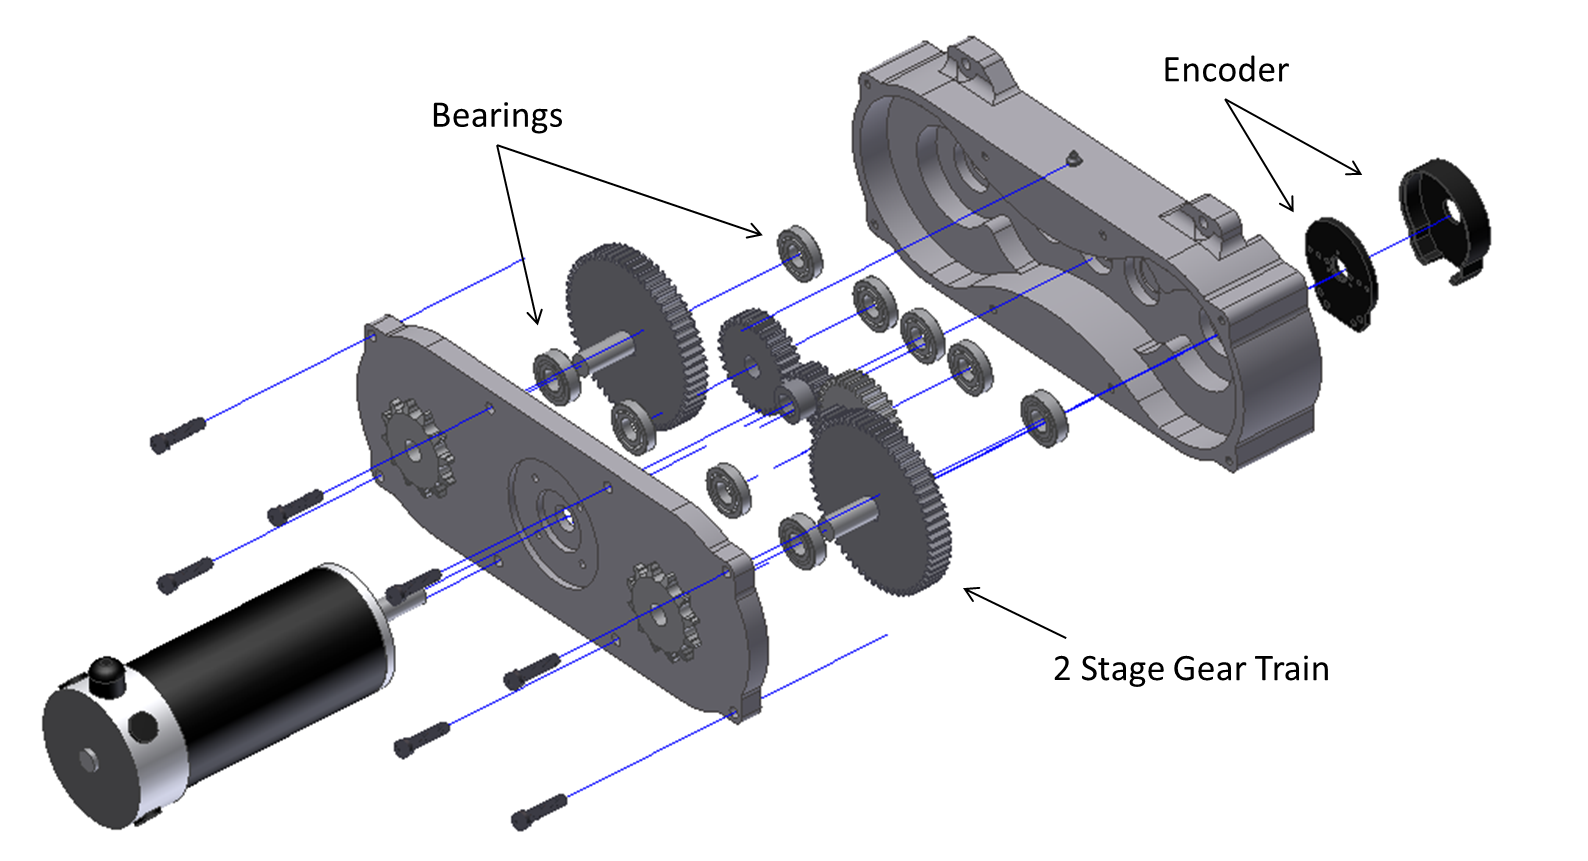
\includegraphics[width=3in]{./Pics/GearboxExploded.png}
\caption{Exploded View of Gearbox}
\label{FIG:Explode}
\end{minipage}
\end{figure}


\subsubsection{Suspension}
The suspension of the robot was greatly improved over the previous year’s design. Prior designs utilized a trailing/leading arm suspension system, connected away from the main body of the robot (see Figure \ref{FIG:Shock}). This year, a four bar linkage mounted to the middle section of the robot was developed in order to reduce the cyclic loading on the frame as well as improve the damping characteristics. Fox DHX RC4 coilover dampers were a much welcomed improvement over previous homemade solutions. The suspension design allows for approximately 5 inches of travel for each wheel, lending the design much superior ride dynamics to ensure stability and dampened impacts while traversing rough terrain.

\begin{figure}[H]
\begin{center}
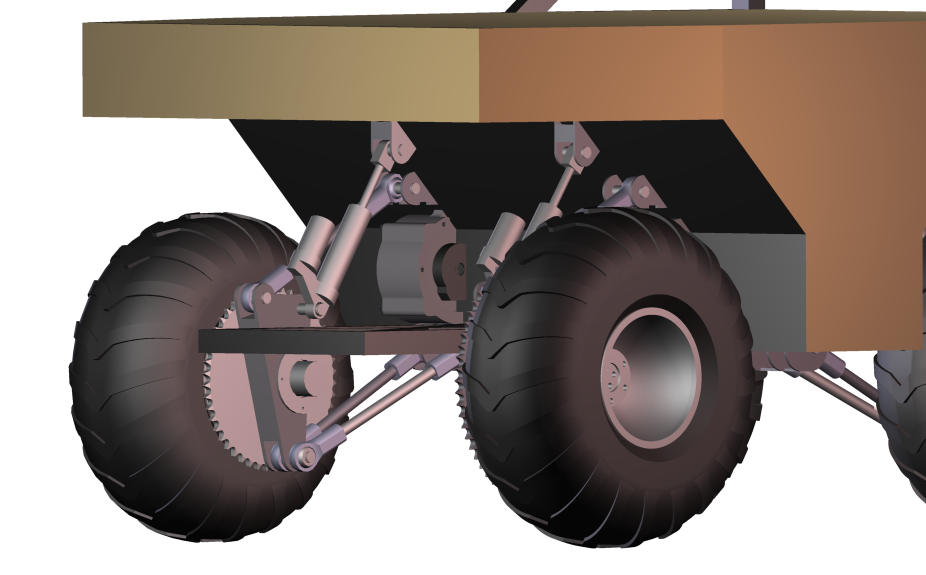
\includegraphics[width=3in]{./Pics/Suspension-Far.png}
\caption{Shock System}
\label{FIG:Shock}
\end{center}
\end{figure}



\subsection{Frame}
The frame is constructed out of 1/16" wall 1" sq. steel tube and aluminum panels. Much of the assembly was accomplished with MIG welding and the use of 1/4-20 fasteners. A model of the frame was made in Siemens NX and finite element analysis was conducted using the NASTRAN package. A stress analysis was performed using half inch tetrahedral elements to determine if the robot would be safe to pick up for maintenance and loading for events. The analysis assumed that the final assembly would have a weight of 500 pounds, overestimating the total weight to give a worst case scenario. When the force to lift the robot was applied to each end, the maximum stresses were found to be 2.33x104 psi. This result is shown in Figure \ref{FIG:stress}.


\begin{figure}[H]
\begin{center}
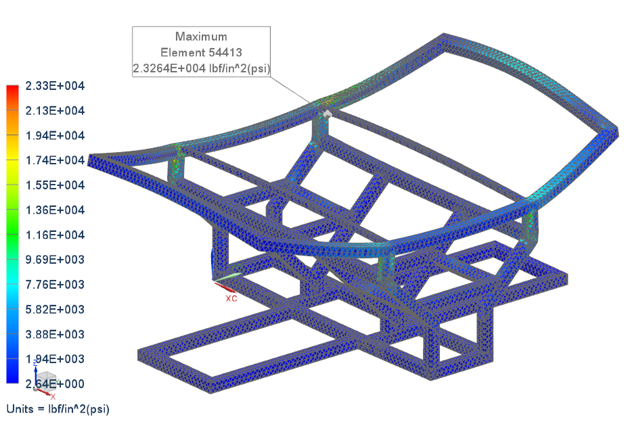
\includegraphics[width=3in]{./Pics/Stress.png}
\caption{Finite Element Streses}
\label{FIG:stress}
\end{center}
\end{figure}

Because this stress is lower than the yield stress of carbon steel of 5x105 psi, a fatigue analysis was conducted to determine how it would behave after one million cycles. Figure \ref{FIG:cycles} shows the number of cycles to failure as predicted by the simulation.

\begin{figure}[H]
\begin{center}
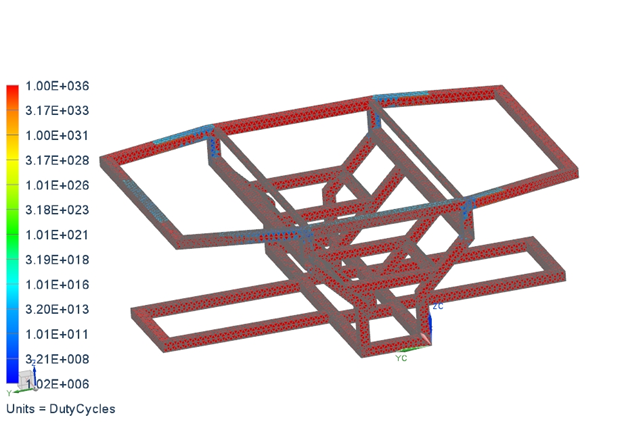
\includegraphics[width=3in]{./Pics/Cycles.png}
\caption{Cycles to Failure}
\label{FIG:cycles}
\end{center}
\end{figure}

The finite element analysis predicted that the frame would last at least 1 million cycles in the worst case scenarios under this loading condition. Also, it predicted a safety factor of 2.89 at the corner where the stresses were highest. Since the model was assumed to be heavier than the true weight and the joints are also reinforced with steel plates, this safety factor is sufficient.
Misti was designed to handle even the roughest of conditions with nearly 8 inches of ground clearance. Using 145/70-6 pneumatic wheels, she can roll over most common obstacles with ease. The larger wheels will improve our ability to traverse small obstacles and climb ramps. While pneumatic tires do offer the potential to go flat, unlike our previous foam core tires, it was determined they would provide a superior ride dynamic and cushion small bumps, particularly at lower speeds.

\subsection{Mast}
A vertical mast on the aft of the robot supports the GPS, IMU, and stereoscopic camera, as well as a button panel for operating the lights, emergency stop and go buttons (Figure \ref{FIG:mast}).
\begin{figure}[H]
\begin{center}
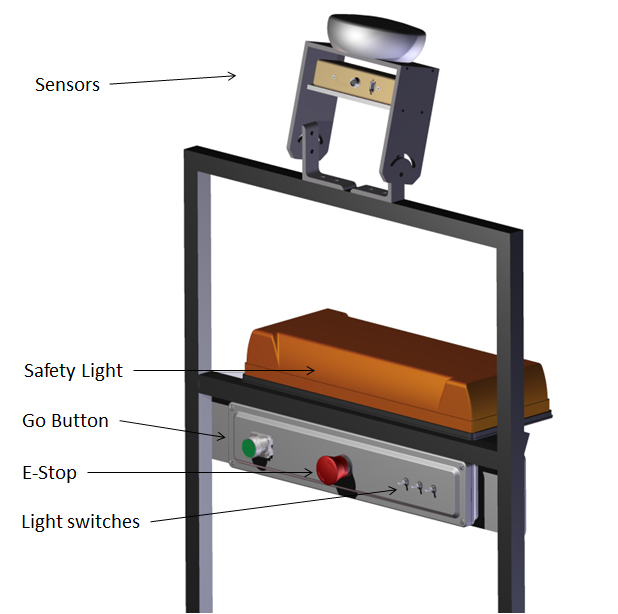
\includegraphics[width=3in]{./Pics/Mast.png}
\caption{Mast}
\label{FIG:mast}
\end{center}
\end{figure}

The mast, which stands 67 inches tall, was designed to give the camera sufficient field of view, while also being just low enough to easily fit inside the RoboJackets’ transportation trailer for ease of travel. The button panel, and particularly the E-stop, resides at forehead height (Figure \ref{FIG:forehead}) with respect to the stance of the user while operating/debugging code onboard computer, a design feature intended to prevent injury in case the robot malfunctions and moves backwards. Components that are exposed to the elements have been weatherproofed by using wash-down enclosures. This provides added robustness, allowing the team to test in inclement weather without worry.
\begin{figure}[H]
\begin{center}
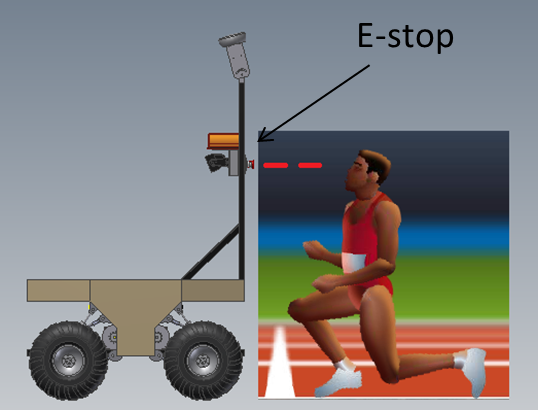
\includegraphics[width=3in]{./Pics/QWOP.png}
\caption{E-Stop at Forehead Height}
\label{FIG:forehead}
\end{center}
\end{figure}

The sensor loadout (Figure \ref{FIG:sensors}) includes a stereoscopic camera, GPS unit, and inertial measurement unit (IMU) on the mast, as well as a LIDAR residing on the bottom of the robot frame and an encoder in each gearbox.

\begin{figure}[H]
\begin{center}
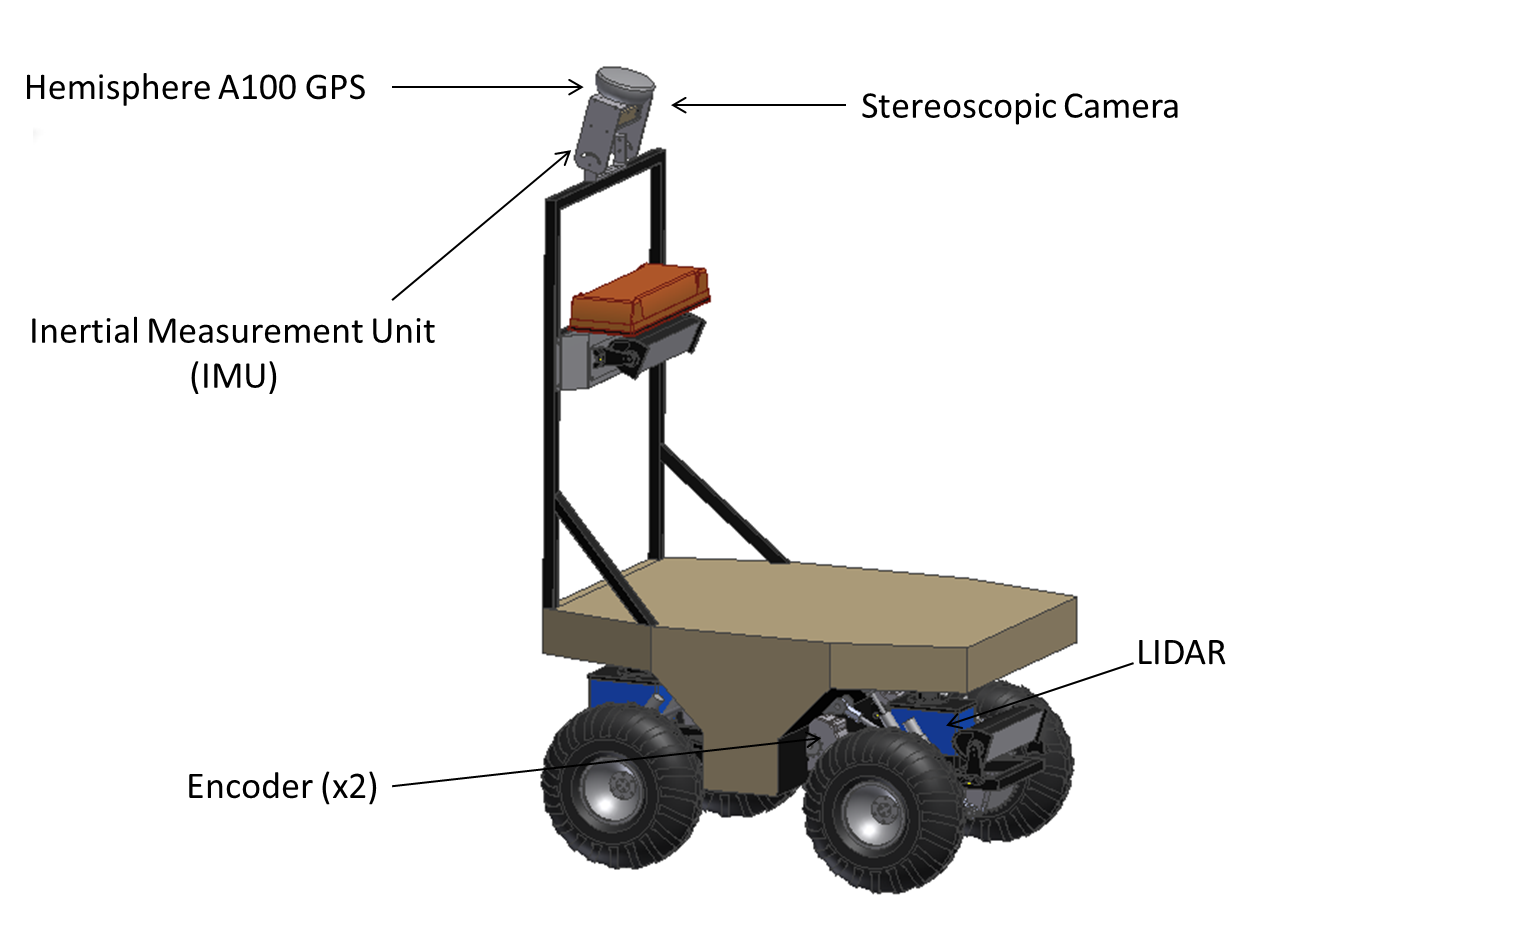
\includegraphics[width=3in]{./Pics/Sensors.png}
\caption{Sensor Loadout}
\label{FIG:sensors}
\end{center}
\end{figure}

To boost safety and night-time/dusk operability, the team installed a large safety light, as well as two large headlights (Figure \ref{FIG:lights}) to light the field both close and far from the vehicle.

\begin{figure}[H]
\begin{center}
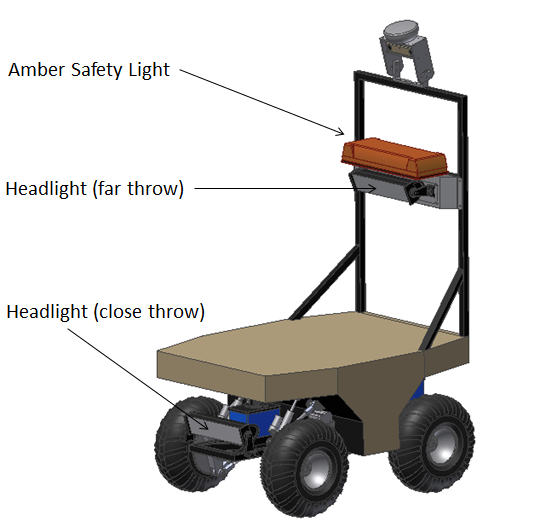
\includegraphics[width=3in]{./Pics/Lighting.png}
\caption{Lights}
\label{FIG:lights}
\end{center}
\end{figure}


\subsection{LIDAR}
% Mention LIDAR FOV protection from rain, accessibility. How it comes off with 3 bolts, etc.
The modified SICK NAV 200 LIDARs are mounted in the front and rear of the vehicle and each have an unobstructed sweep of roughly 255 degrees. The LIDARs are protected above from rain by overhangs which also serve as compartments for the laptop and electrical power system. The units are attached to the base through an intermediate aluminum plate. This allows them to be removed from the vehicle with only loosening three 1/4-20 bolts which are the standard fastener for our platform.
